\textbf{\textcolor{blue}{5.}} \Large
A partir del Ejercicio 4, muestra los registros de activación generados por la función con
la siguiente llamada.
\begin{lstlisting}
(ocurrencias '(1 2 3) '(1 2))
\end{lstlisting}

\textbf{Solución.} Al igual que en el ejercicio 3, las llamadas recursivas son las mismas\footnote{11 registros
más la llamada a la función \code{cola\_ocurrencias} que genera un registro extra, en total 12 registros.}
exceptuando las modificaciones en el nombre de las respectivas funciones y la manera en la que se guarda el acumulador,
acontinuación presentamos como se ve el último registro de activación al llama la función con los valores indicados, esto es
                   
%%%%%%%%%%%%%%%%%%%%%%%% Último Registro:
%\begin{table}[h]
%        \centering
%       \renewcommand{\arraystretch}{1.5}
%        \begin{tabular}{ | c | c }
%                         Resultado:                       &     \\
%                         \code{'((() 1 . 1) 2 . 1)}       & 0x50\\
%                         \hline
%                         Cuerpo/definición                & 0x51\\
%                         \hline
%                         \code{'()}                       &     \\
%                         \code{'(1 2 3)}                  & 0x50\\
%                         \hline
%                         \code{ocurrencias\_cola}         & 0x49\\
%                         \hline
%        \end{tabular}
%\end{table}

\begin{center}
        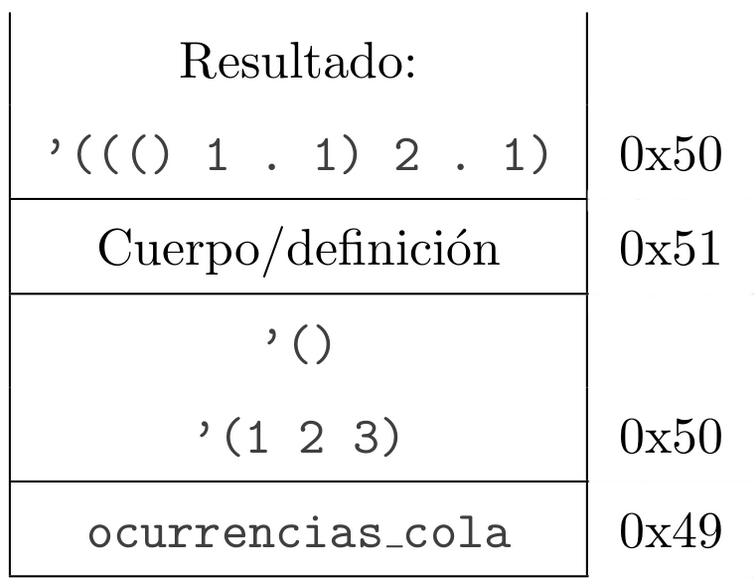
\includegraphics[scale=0.25]{./Ultimo}
\end{center}
